\subsection{Towards NNLO with full top quark mass dependence}

%\textit{Authors:} Joshua Davies, Kay Sch\"onwald, Matthias Steinhauser, Marco Vitti

\textbf{Joshua Davies, Kay Schönwald, Matthias Steinhauser, Marco Vitti~\cite{Davies:2023obx,Davies:2024znp,Davies:2025ghl}.}

\noindent In order to increase the precision for the theoretical prediction of double Higgs boson production and tackle the large uncertainties due to the top quark mass renormalization scheme, one needs information about higher-order corrections to the process.
This can be achieved either by resummation of large logarithms in certain kinematic regions, see Section~\ref{sec:scet}, or by calculating the higher-order corrections directly.
There is an ongoing effort to compute the virtual NNLO corrections to double Higgs boson production retaining top quark mass effects beyond the large mass expansion.


The computation of the NNLO amplitude can be split into several building blocks of differing complexity, shown in Fig.~\ref{fig::gghh_FDs}.
The one-particle reducible contributions, see Fig.~\ref{fig::gghh_FDs}(a), which are only of one-loop times two-loop complexity, have been calculated in Ref.~\cite{Davies:2024znp} for general kinematics.
The calculation of the genuine three-loop contributions faces technical challenges due to the large number of loops and scales.
They are addressed using an expansion in $p_T$ or, equivalently, $m_h$ and $t$.
The first expansion terms have been obtained for the contributions including a closed light quark loop, see Fig.~\ref{fig::gghh_FDs}(b), and, in the large-$N_c$ limit, for the diagrams involving one closed top quark loop, see Fig.~\ref{fig::gghh_FDs}(c); here $N_c$ stands for the number of colours in QCD.
In these works, amplitude processing, expansion and IBP reduction were performed with {\tt FORM} \cite{Ruijl:2017dtg,Davies:2026cci}, {\tt Feynson} \cite{Maheria:2022dsq}, {\tt Kira} \cite{Lange:2025ofh} and {\tt FIRE} \cite{Smirnov:2025prc}.
The class of diagrams represented in Fig.~\ref{fig::gghh_FDs}(d), which involves two top quark loops, faces the additional challenge of massless cuts in the $t$-channel or isolating an external Higgs boson and therefore requires a more involved asymptotic expansion.
They are not yet known, but remain work in progress.

At LO and NLO the first expansion term in the forward limit provides an approximation with an accuracy at the 20\% level for $p_T < 300 \,$GeV (see, e.g., Ref.~\cite{Davies:2025ghl}).
Therefore, one can use these results to study the dependence on the top quark mass renormalization scheme at NNLO.
In Fig.~\ref{fig::G1_ratio} we show the quantity
$|G_{\rm box1}|^2$, where $G_{\rm box1}$ is the box contribution of the properly normalized form factor $F_1$
(see Ref.~\cite{Davies:2025ghl} for details)
normalized to the three-loop result in the on-shell scheme as a function
of partonic $\sqrt{s}$. The bands for the $\overline{\rm MS}$ results arise from the variation of the renormalization scale
associated with the top quark mass. The two panels correspond to two different choices of $\mu_s$, the renormalization scale of $\alpha_s$.
One observes a good convergence of the perturbative expansion
in both renormalization schemes.
One also observes smaller perturbative corrections when using the $\overline{\mathrm{MS}}$ scheme for the top quark mass and a shrinking of the scale uncertainty bands. Furthermore, the
NNLO predictions are closer together than the corresponding curves at lower orders. All of these are very encouraging features.

A full NNLO analysis also needs the top quark mass dependence of the real radiation amplitudes.
While the one-loop amplitudes with two additional real emissions can be obtained with automated tools, the two-loop amplitudes with one additional real emission are not known yet and constitute another computational challenge.

\begin{figure}[t]
    \begin{center}
    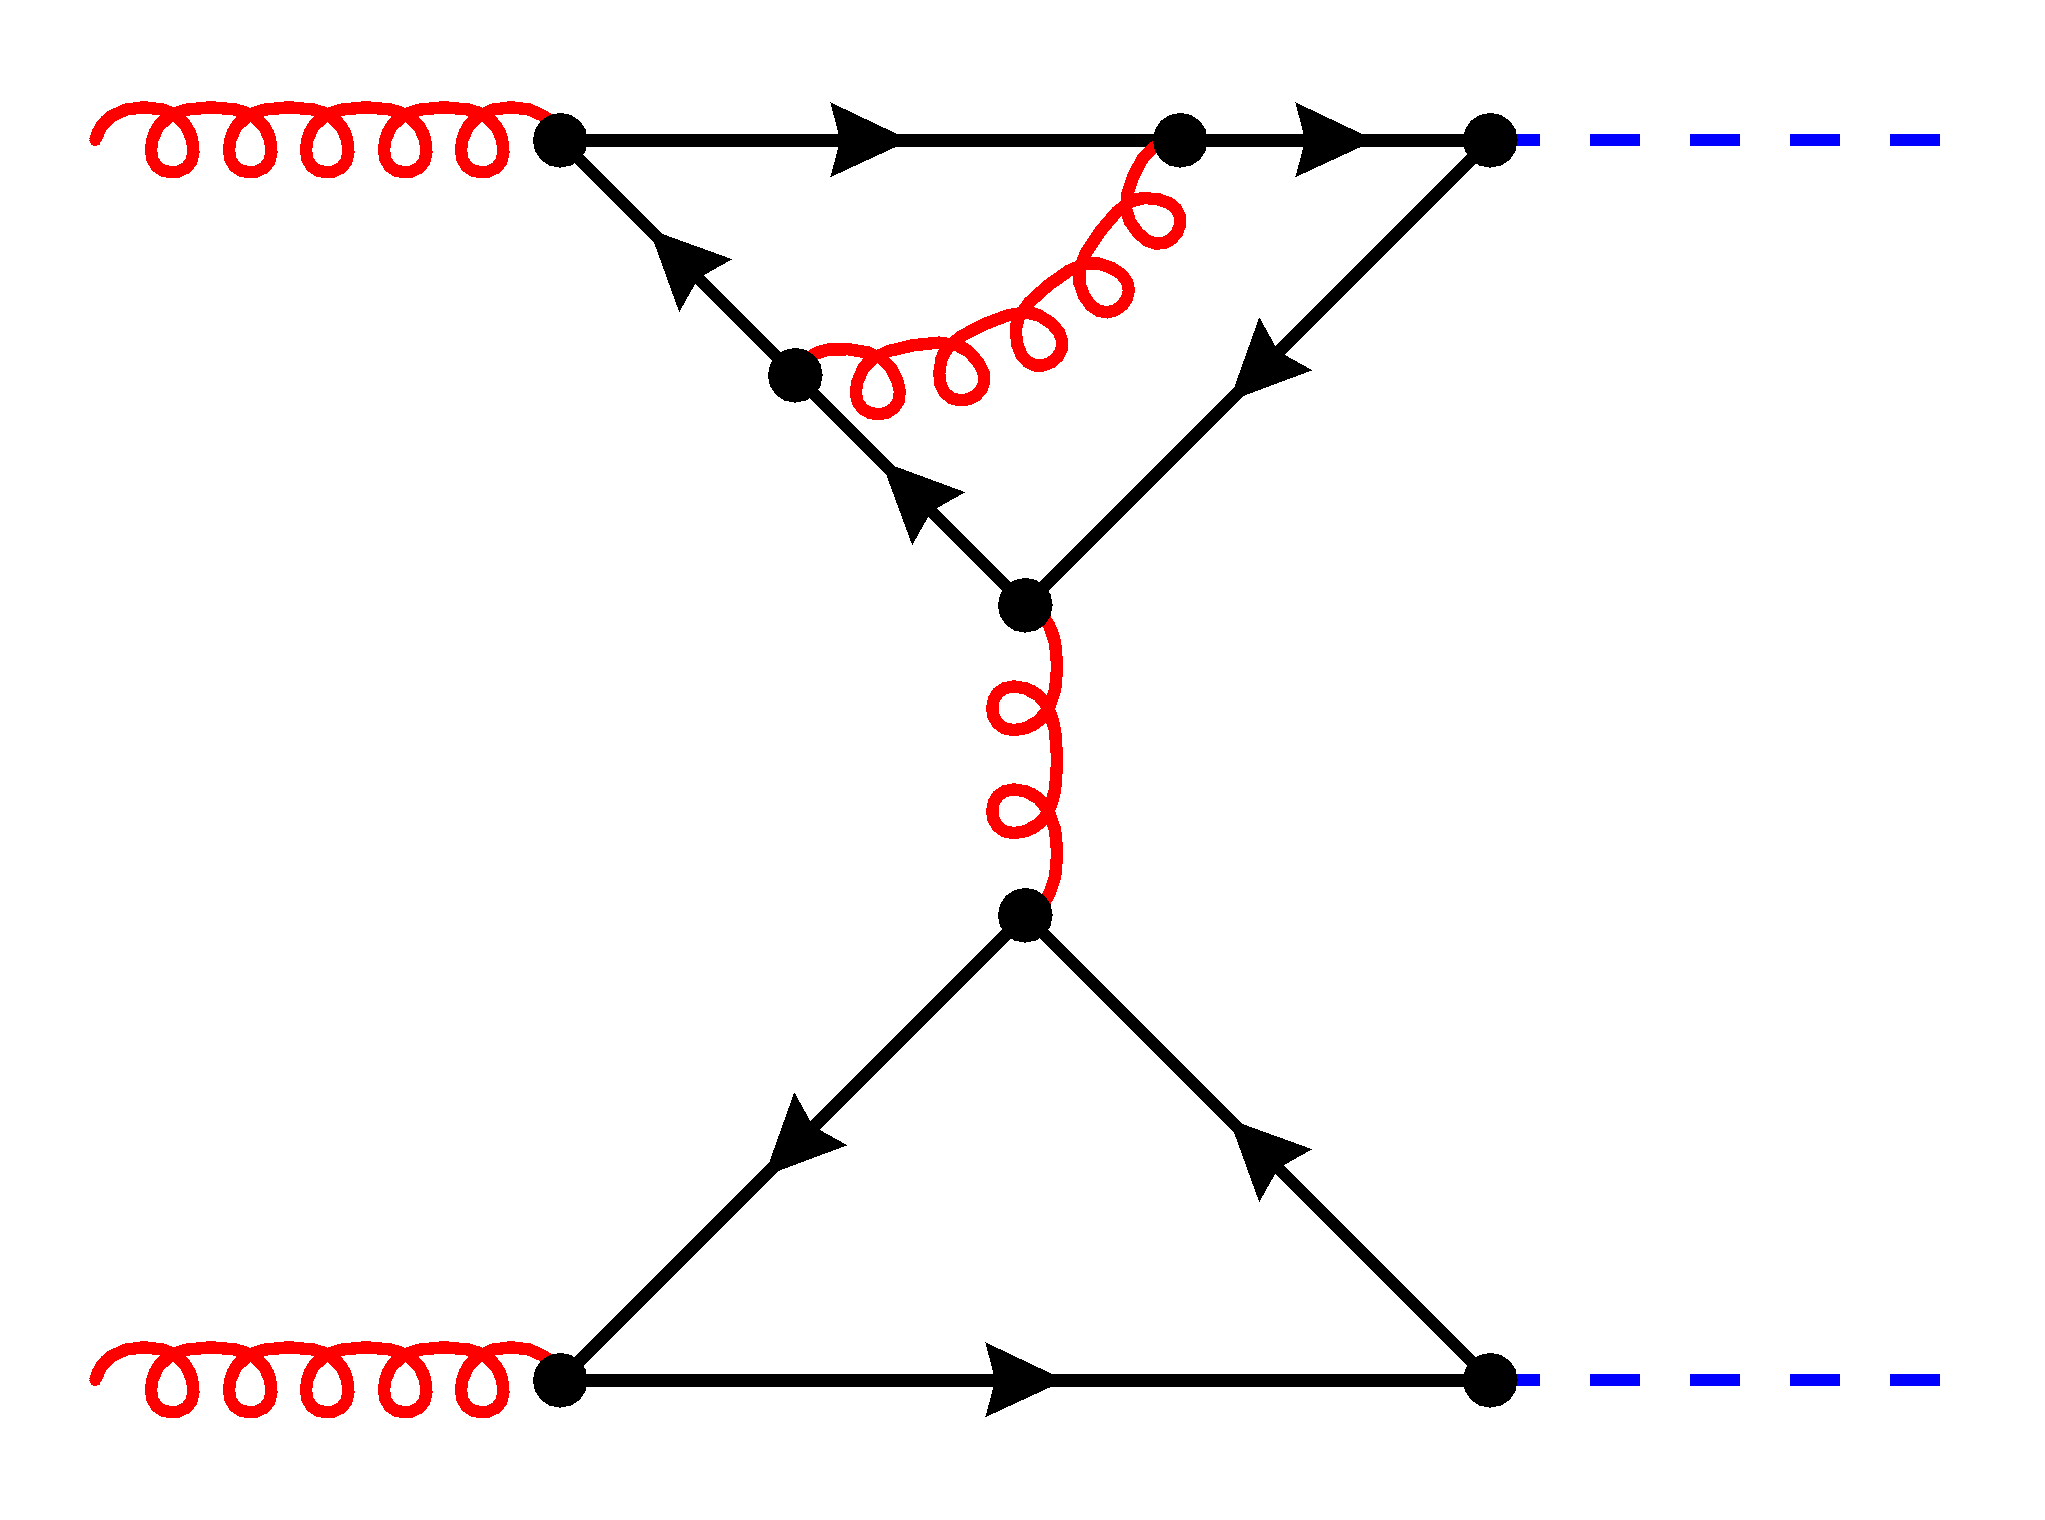
\includegraphics[width=.24\textwidth]{NNLO_QCD_SM/NNLOmt/Images/reducible}
    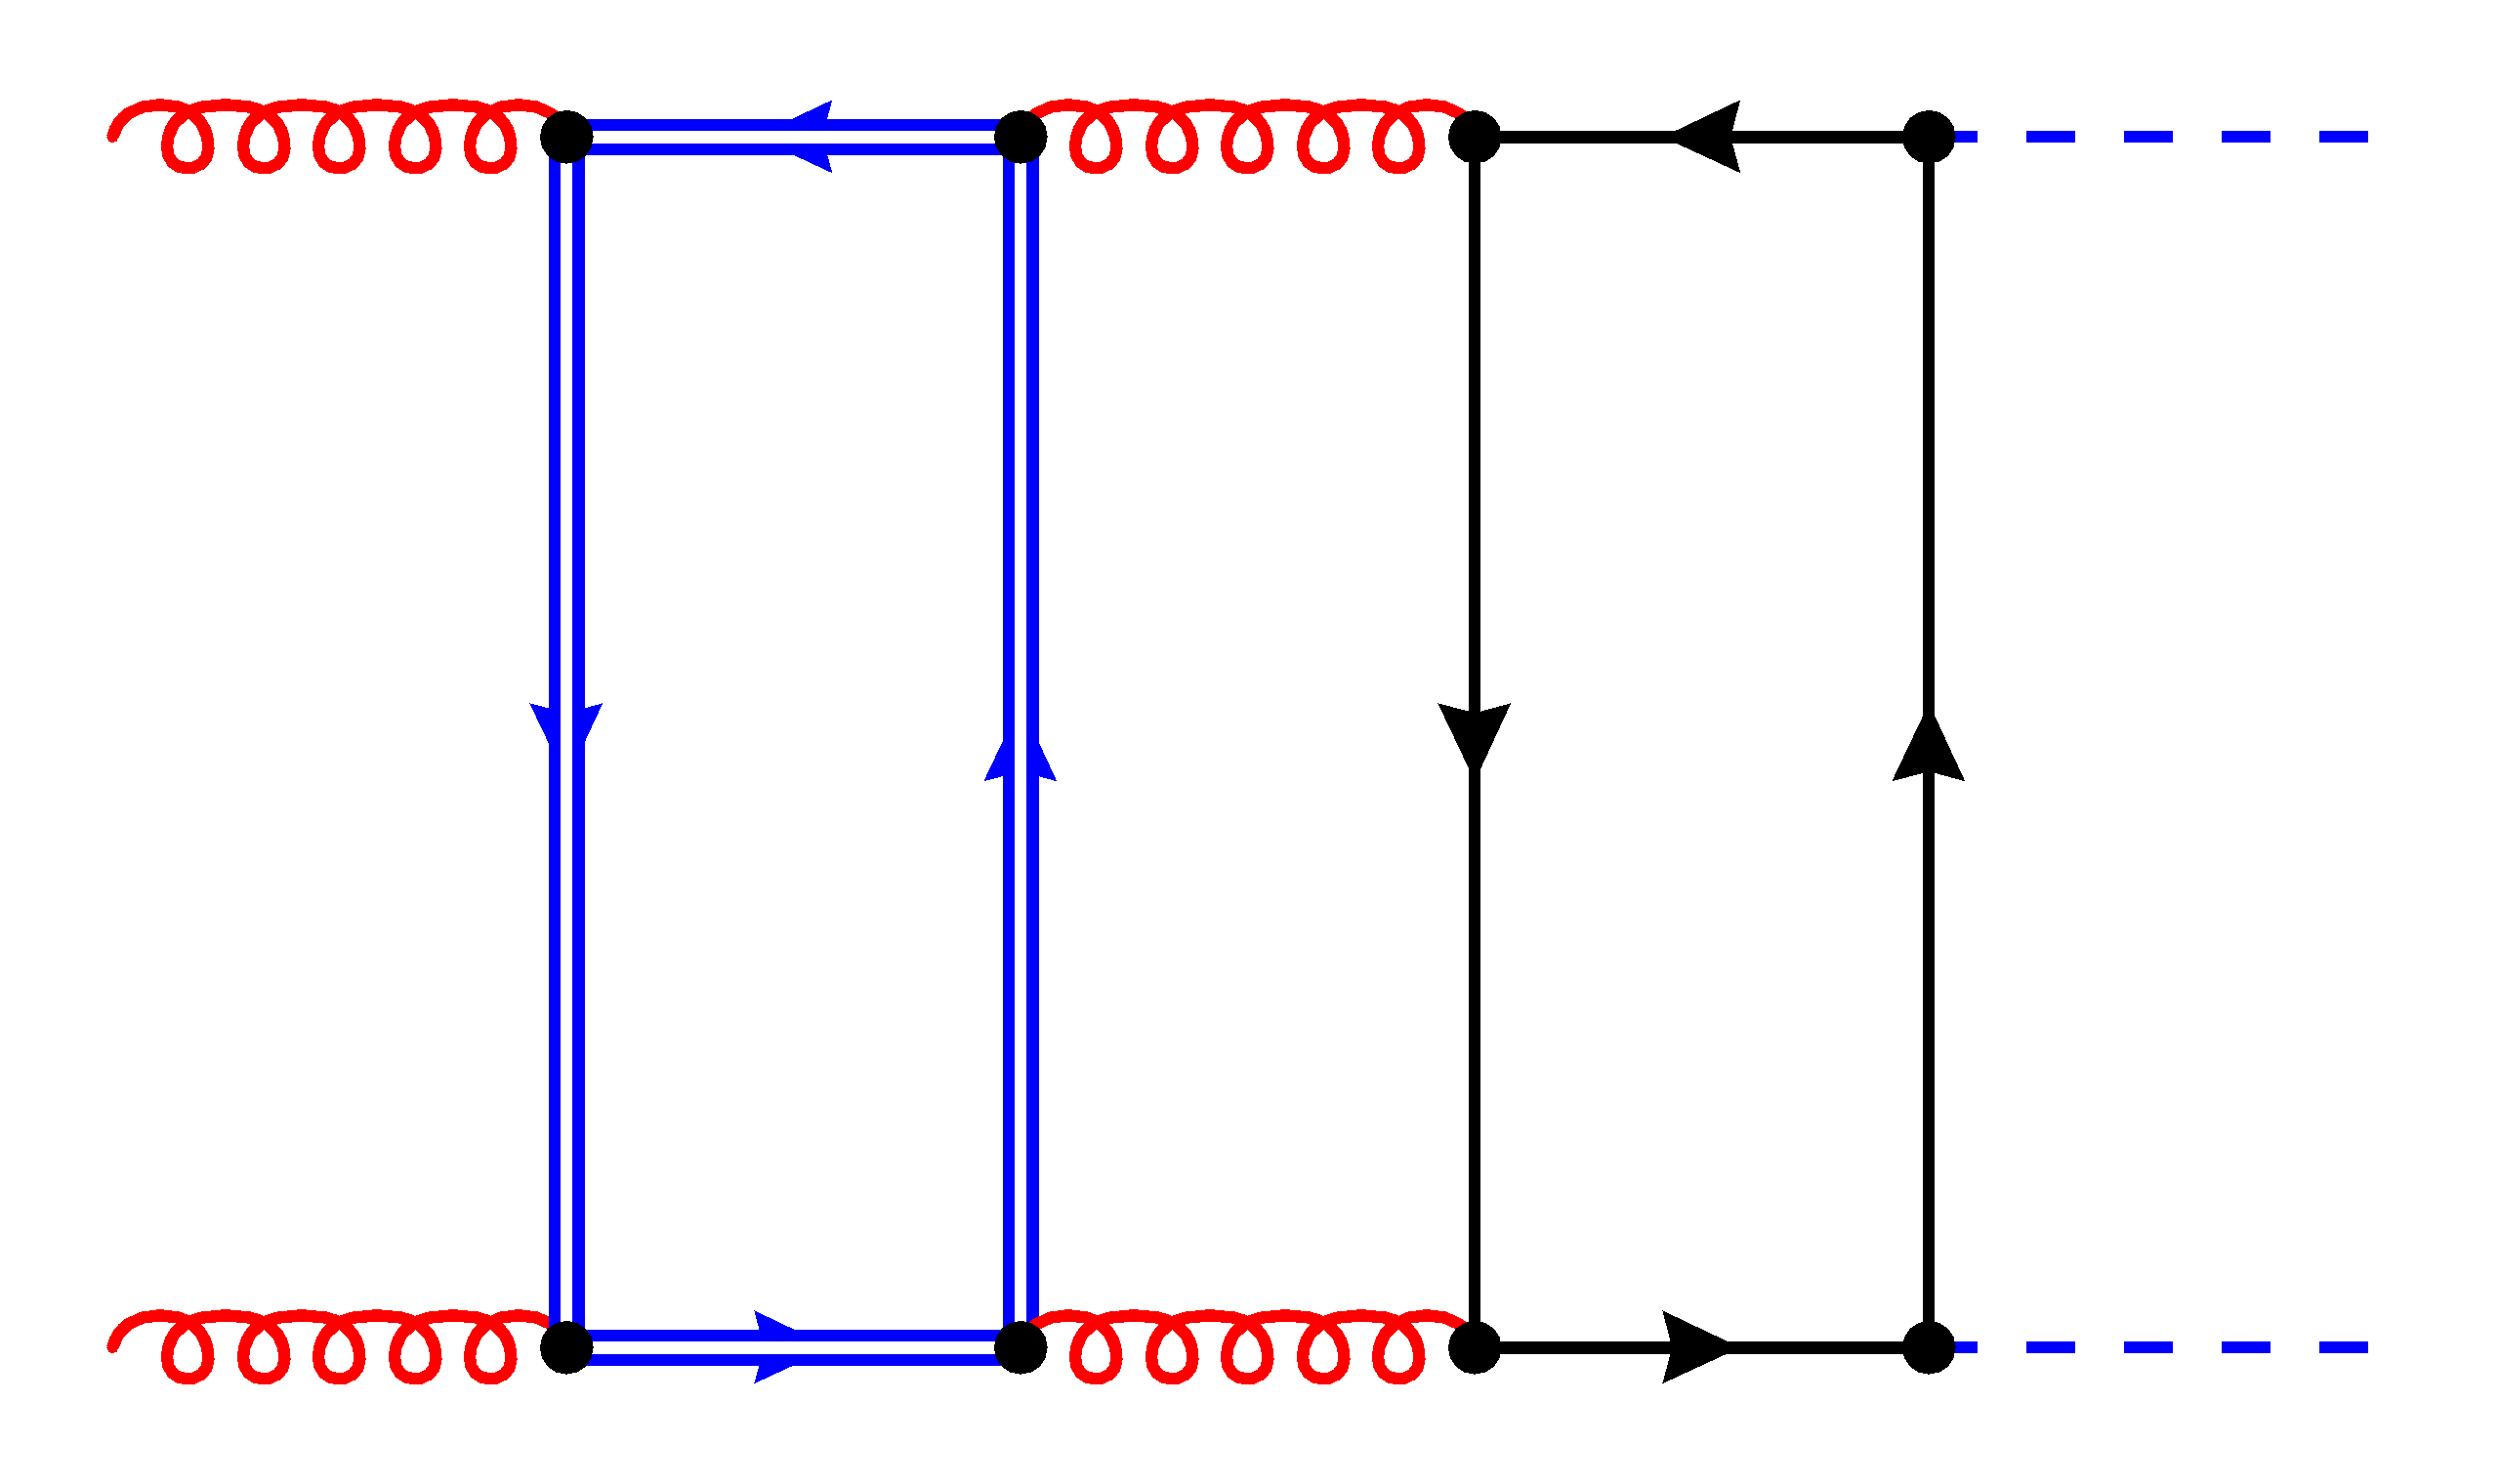
\includegraphics[width=.25\textwidth]{NNLO_QCD_SM/NNLOmt/Images/nl}
    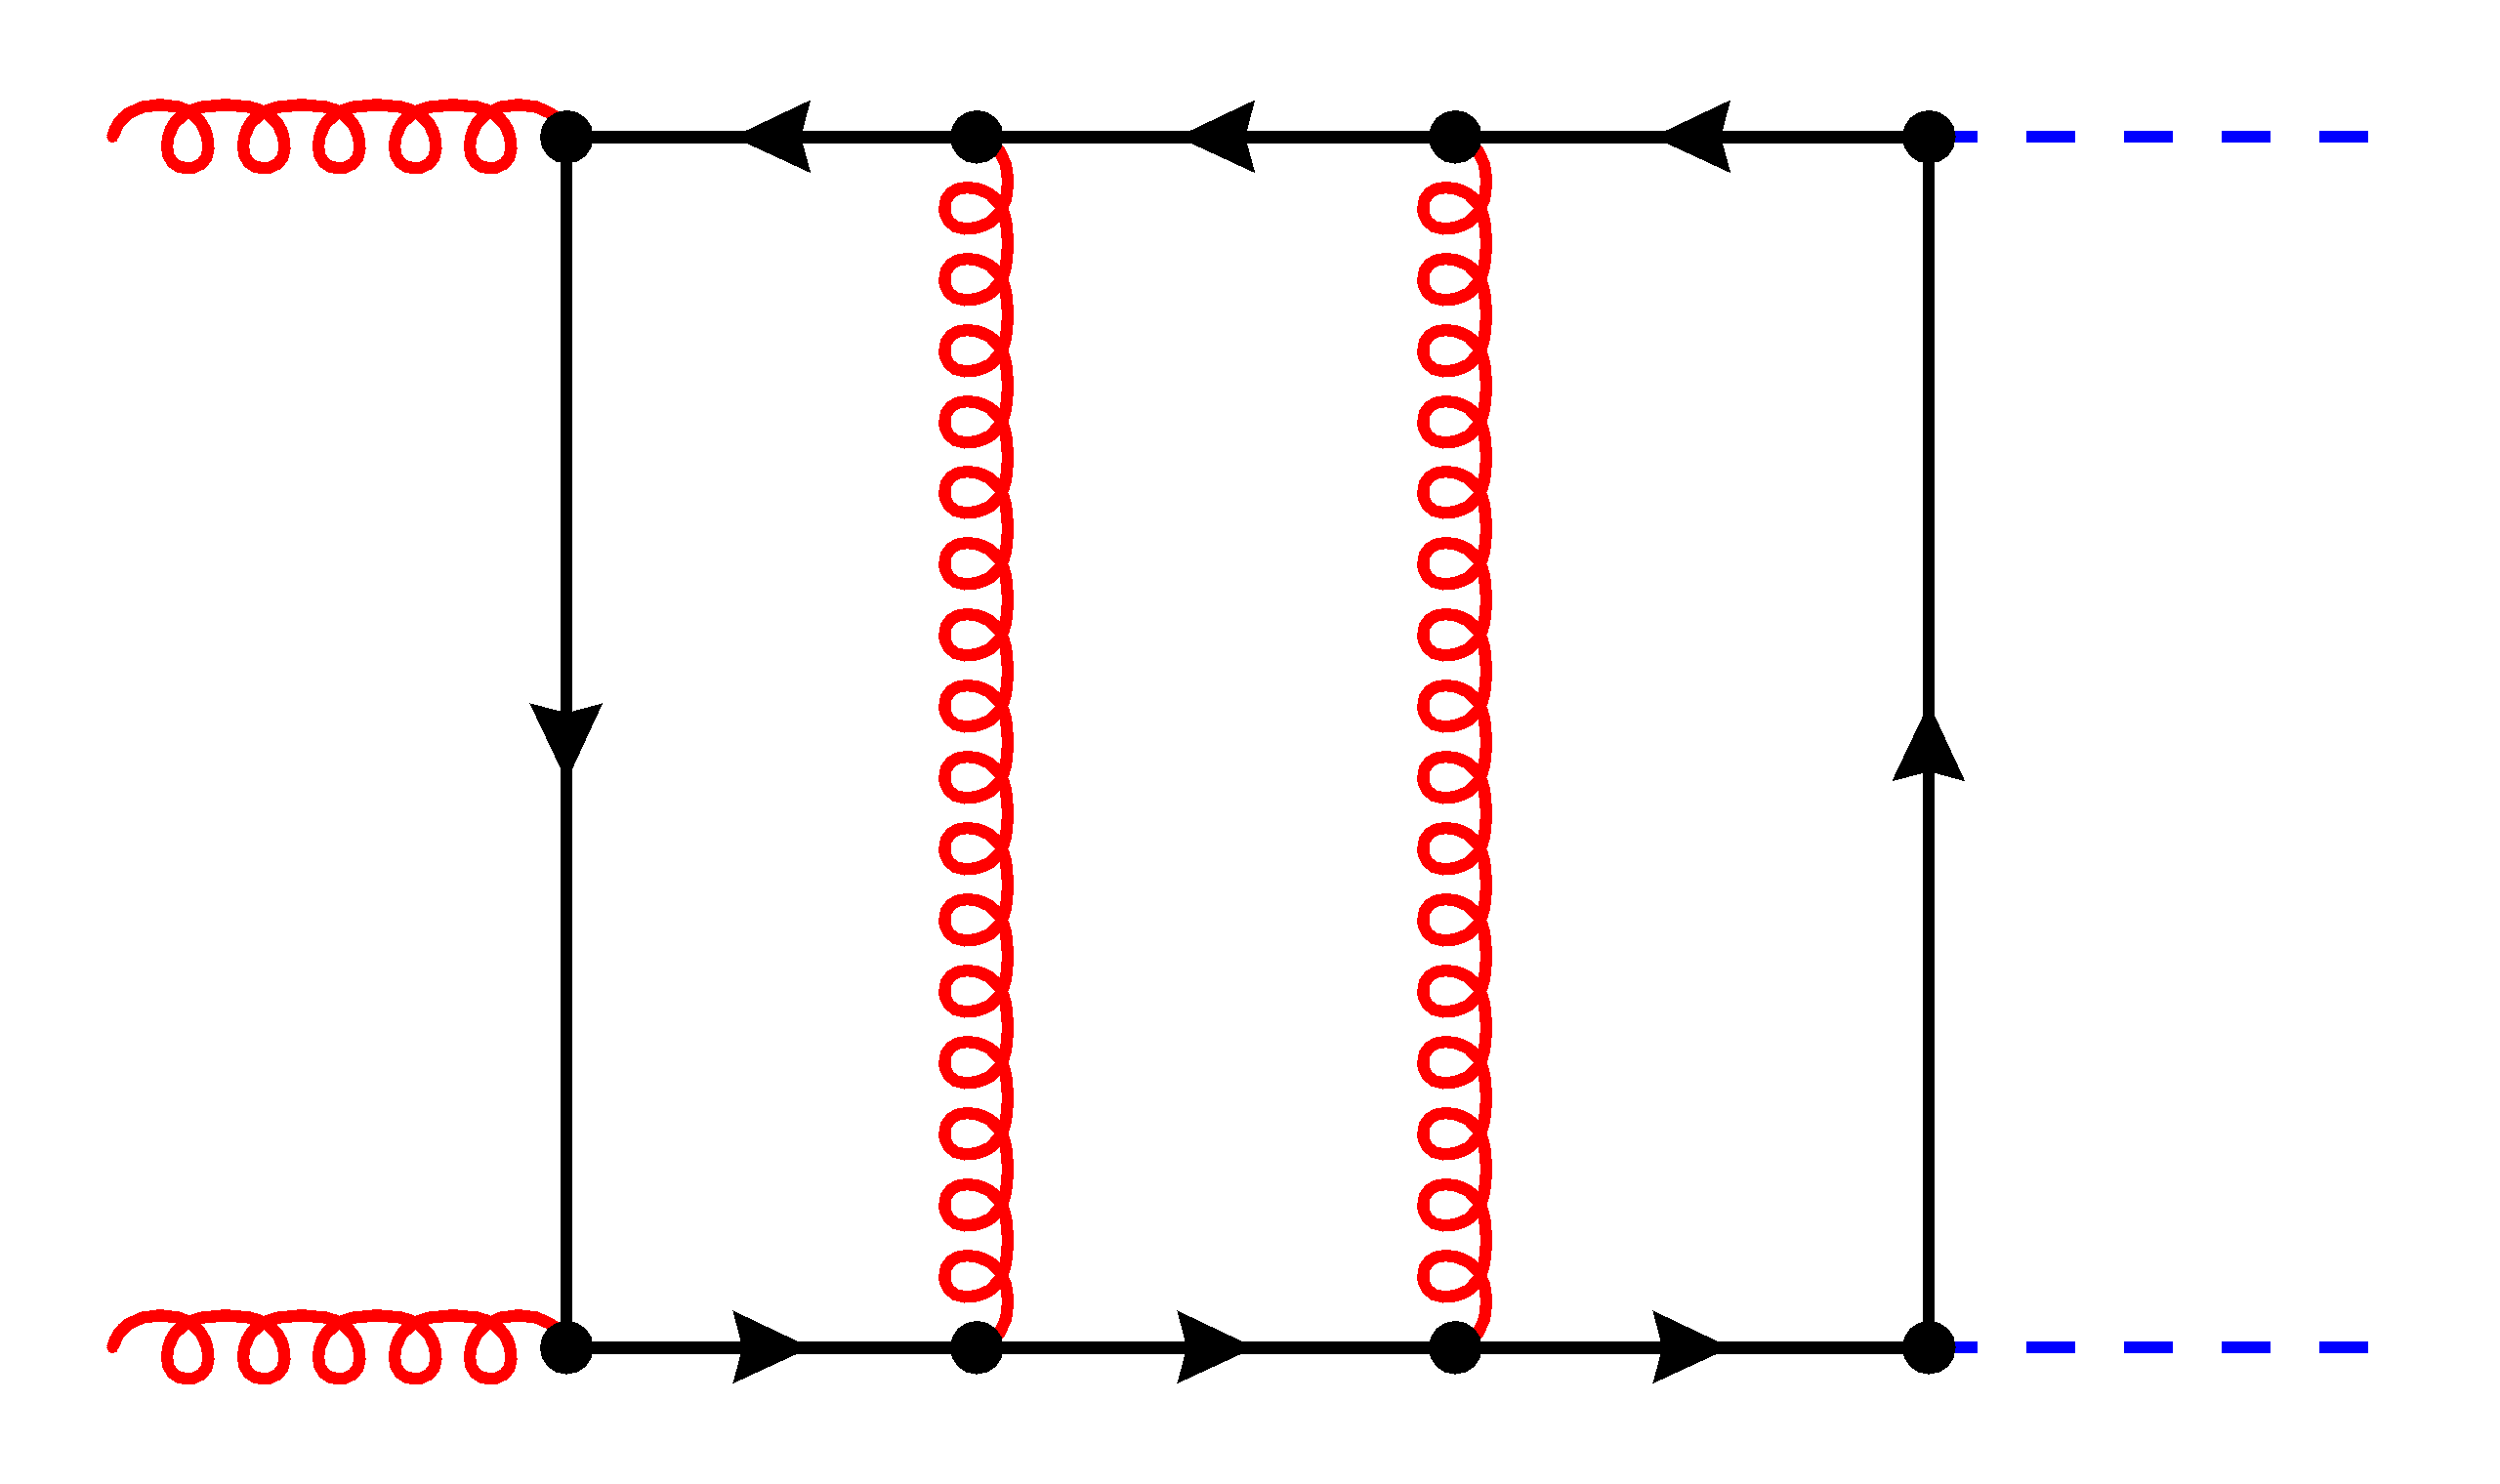
\includegraphics[width=.25\textwidth]{NNLO_QCD_SM/NNLOmt/Images/nh-1}
    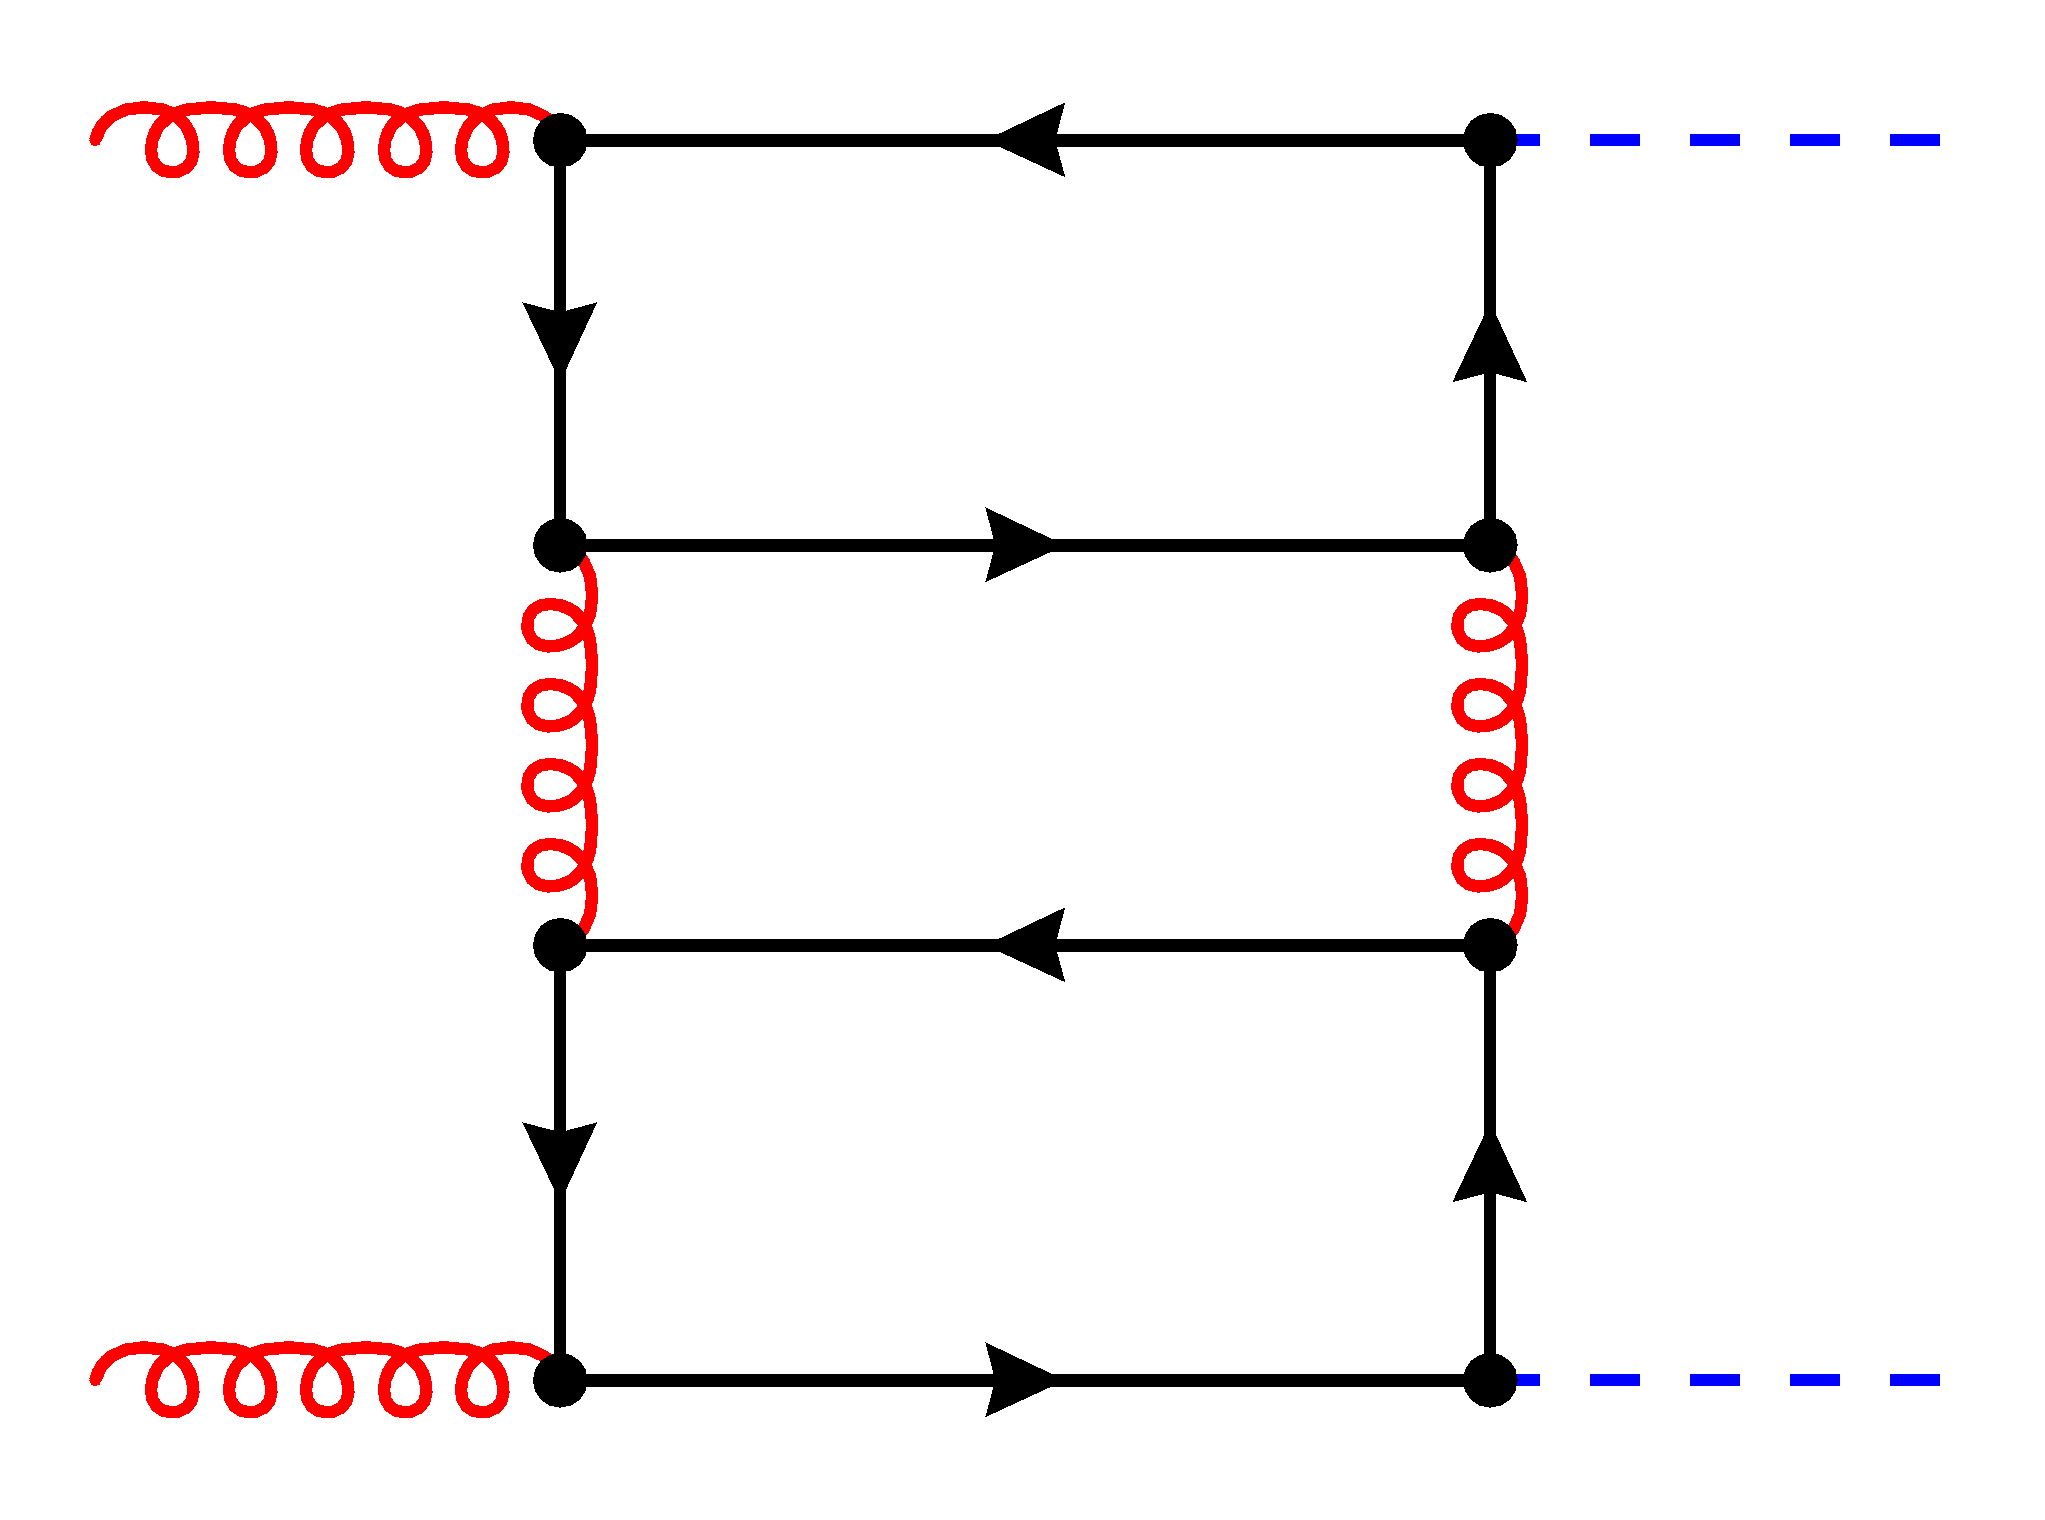
\includegraphics[width=.24\textwidth]{NNLO_QCD_SM/NNLOmt/Images/nh2}
    (a)
    \hspace{0.2\textwidth}
    (b)
    \hspace{0.2\textwidth}
    (c)
    \hspace{0.2\textwidth}
    (d)
    \end{center}
  \caption{\label{fig::gghh_FDs}Sample Feynman diagrams of contributions to the virtual NNLO corrections.
  The contributions shown represent: (a) reducible contributions,
  (b) contributions with one closed light quark loop,
  (c) contributions with one closed top quark loop,
  (d) contributions with two closed top quark loops.
  Curly (red) lines correspond to gluons,
  single (black) lines to the top quark,
  double (blue) lines to a massless quark
  and dashed (blue) lines to the Higgs boson.
  The diagram classes follow Refs.~\cite{Davies:2023obx,Davies:2024znp,Davies:2025ghl}.
  }
\end{figure}

\begin{figure}[H]
\begin{center}
  \begin{tabular}{cc}
    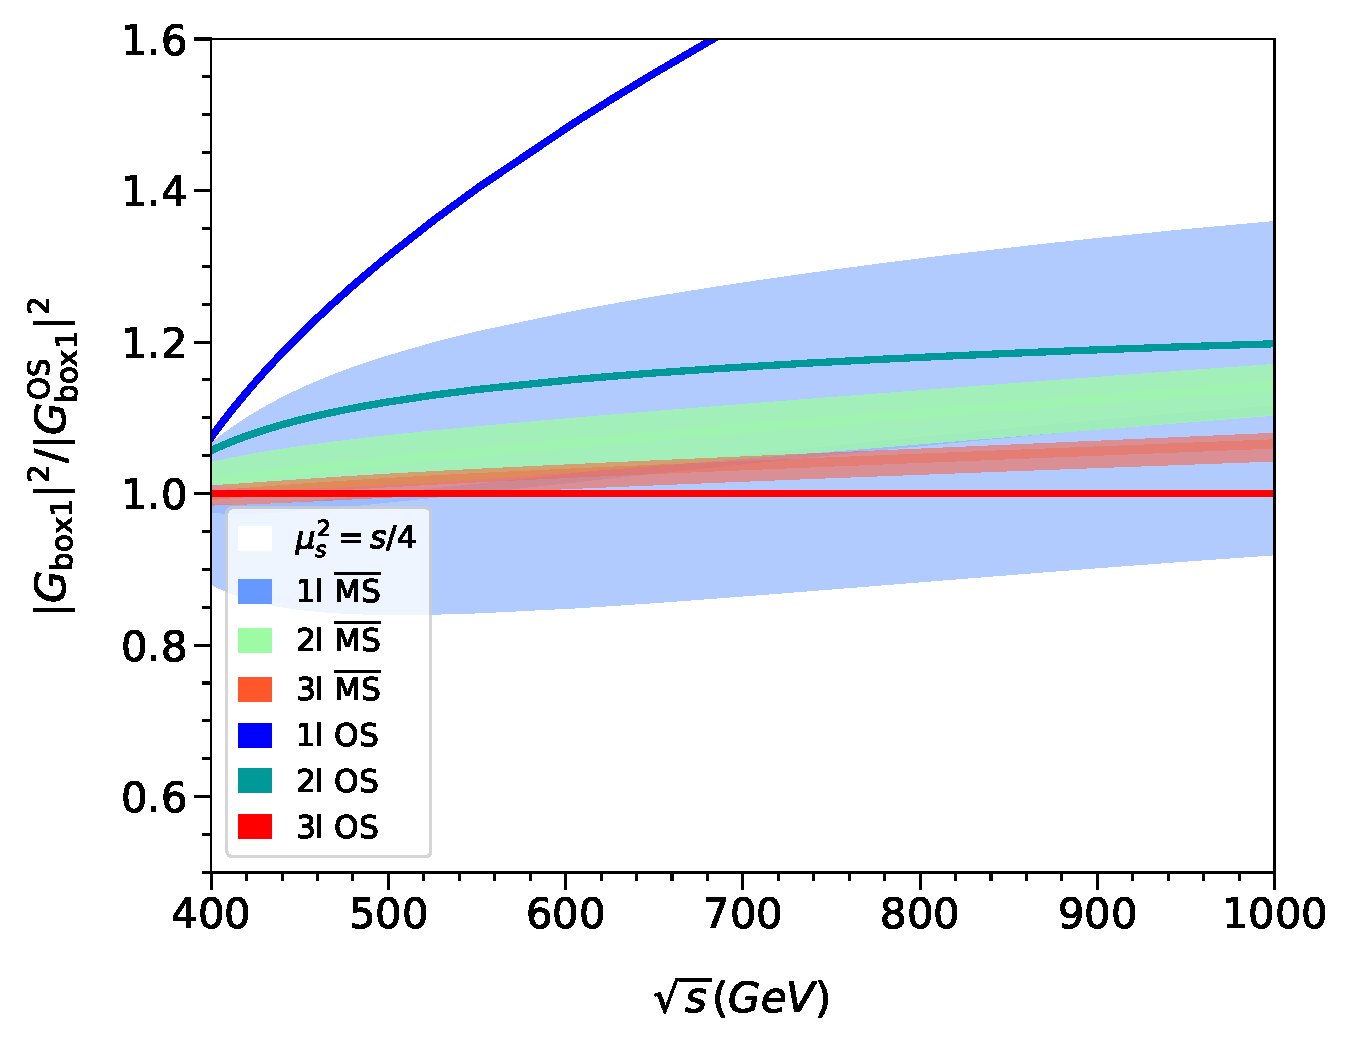
\includegraphics[width=0.45\textwidth]{NNLO_QCD_SM/NNLOmt/Images/ratio1_abs_musso4.pdf}
    &
    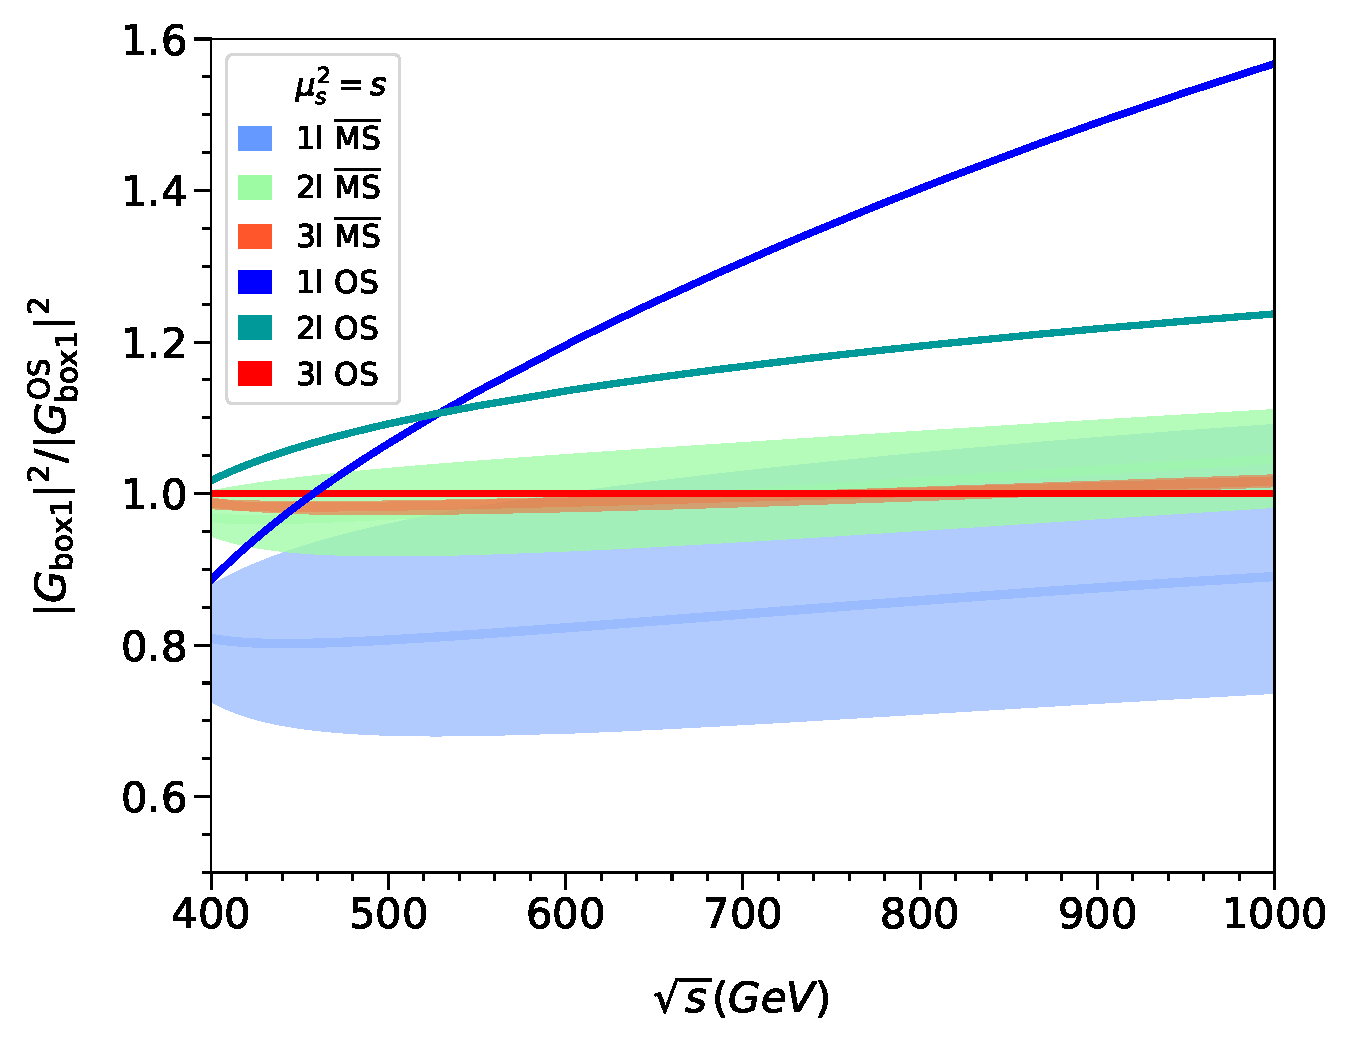
\includegraphics[width=0.45\textwidth]{NNLO_QCD_SM/NNLOmt/Images/ratio1_abs_muss.pdf}
  \end{tabular}
\end{center}
  \caption{\label{fig::G1_ratio} $G_{\rm box1}$
  computed with the $\overline{\rm MS}$ and on-shell
  definition of the top quark mass for
    $\mu_s^2=s/4$ (left) and $\mu_s^2=s$ (right). $\mu_t^2$ is chosen between $s$ and $s/16$. All curves are normalized to the three-loop on-shell result. Results shown are from Ref.~\cite{Davies:2025ghl}.}
\end{figure}
